% This report template is adapted from the IEEE style.
% https://www.ieee.org/conferences/publishing/templates.html

\documentclass[conference]{IEEEtran}
\IEEEoverridecommandlockouts


% TODO commands package
\usepackage{todonotes}
\newcommand{\pe}[1]{\todo[inline, backgroundcolor=green]{PE: #1}}
\definecolor{eyecancerpink}{rgb}{1.0, 0.0, 1.0}
\newcommand{\nm}[1]{\todo[inline, backgroundcolor=eyecancerpink]{NM: #1}}

\usepackage{cite}
\usepackage{amsmath,amssymb,amsfonts}
\usepackage{algorithmic}
\usepackage{graphicx}
\usepackage{textcomp}
\usepackage{xcolor}
\usepackage{tikz}
\usepackage{hyperref}
\usepackage{float}
\def\BibTeX{{\rm B\kern-.05em{\sc i\kern-.025em b}\kern-.08em
    T\kern-.1667em\lower.7ex\hbox{E}\kern-.125emX}}


% Multi-column list
\usepackage{multicol}


\begin{document}

\title{Towards Language Model-based Identification of Business Clusters}

\author{\IEEEauthorblockN{1\textsuperscript{th} Müller Nicola}
\IEEEauthorblockA{s8namuel@stud.uni-saarland.de \\ 2578753}
\and
\IEEEauthorblockN{2\textsuperscript{st} Leist Robert}
\IEEEauthorblockA{s8roleis@stud.uni-saarland.de \\ 2580448}
\and
\IEEEauthorblockN{3\textsuperscript{nd} Eichler Paul}
\IEEEauthorblockA{s8pleich@stud.uni-saarland.de \\ 2578569}
\and
\IEEEauthorblockN{4\textsuperscript{rd} Recktenwald Tobias}
\IEEEauthorblockA{s8tsreck@stud.uni-saarland.de \\ 2577468}
\and
\IEEEauthorblockN{5\textsuperscript{th} Nazari Hameed}
\IEEEauthorblockA{abna00001@stud.uni-saarland.de \\ 7004543}
}

\maketitle

\begin{abstract}
	One of the most important decisions every business has to decide on is a physical location. Identifying the right location is crucial for effective marketing strategies to reach the intended customer base. It can also reduce transportation costs, and locating in a vibrant regional business cluster can significantly positively affect business development.
	However, strategically acquiring \& analyzing data on regional economies, the affiliated companies, and their target market segments is very complex and labor-intensive. 
	
	We propose to circumvent these challenges by leveraging state-of-the-art language models to transform publicly available company websites into machine-readable data points and applying clustering to make location recommendations for novel companies.
	
	A qualitative evaluation of our methods being applied to data from the German municipality Saarland demonstrates that our methods can accurately cluster related companies and categorize novel companies into existing clusters.
\end{abstract}


\section{Introduction}

Deciding on the location of a business is a vital strategic decision. Finding the right location can have several benefits: First, it is crucial for most businesses to be located close to their customers and suppliers for more effective marketing or reduced transportation costs. Secondly, being located in an active regional cluster can significantly benefit a business development \cite{clustersandcomp,gems-model, regionaladv, clustertheory}. 

Business clusters are local concentrations of businesses, manufacturers, suppliers, and institutions from the same field. Identifying business clusters is done by combining geographical data of companies' locations with information on their corresponding market segments. This geographic proximity of related businesses enables efficient cooperation and knowledge transfer, which has been shown to significantly increase the productivity of all businesses within the cluster \cite{clustersandcomp,gems-model, regionaladv, clustertheory}. Thus, establishing or further developing business clusters is of high interest to companies and local governments. Therefore, significant effort is spent identifying clusters and market segments in regional economies. 

However, the identification of market segments, and moreover that of business clusters, requires a significant amount of manual labor. Typically, one must first collect information about companies with a location in the targeted region. Afterward, for each company, their publicly available information must be analyzed to understand their products, strategic position, and market positioning. 

This process is very labor-intensive, as businesses do not provide specific data on the latter points, but it must be inferred from their product portfolio and websites. Additionally, even basic data like the number of employees is often unavailable or difficult to extract automatically, especially for small regional companies.

At the same time, recent advances in natural language processing (NLP), e.g., the popular ChatGPT \cite{chatgpt}, have yielded surprisingly good results in numerous applications. Especially they have proven to be very efficient at extracting data and summaries from human written texts.

The main contribution of this work is an automatic clustering pipeline to effectively identify market segments and business clusters from publicly available information. Utilizing those clusters, our system can provide a strategic location recommendation, which we will demonstrate by using the German federal state Saarland as an example. The novelty of our approach is that we rely on language models to process the companies' information. 

Our clustering pipeline can be divided into $4$ distinct steps: $1)$ gathering descriptions from the websites of companies, $2)$ computing embeddings of the text data, $3)$ reducing the embeddings' dimensionality, and $4)$ applying clustering algorithms.

$1)$ To construct data points for companies in Saarland, we rely on publicly available descriptions from their websites, allowing us to circumvent the challenges of gathering economic data. Since these descriptions are intended to attract customers and investors, they contain all relevant information for characterizing the companies.

$2)$ Given the company descriptions, we utilize state-of-the-art language models to compute embeddings of the text data, corresponding to low-dimensional vectors encompassing the data's essential information. 

$3)$ We further reduce the dimensionality of the embeddings using non-linear dimensionality reduction techniques, which enables us to preserve the non-linear relationships between the embedded text data while avoiding the curse of dimensionality. 

$4)$ Lastly, we apply well-established clustering algorithms in the low-dimensional feature space to assign each company to a cluster from which a potential market segments can be inferred.

Our location recommendation system builds upon the clustering pipeline by computing an embedding of a novel company's description, assigning it to a cluster, and then identifying the most similar companies within the cluster. The system then recommends that the novel company locate its site near an established company acting in the same market segment, which fosters business cluster development in Saarland.

We provide a graphical user-interface for our methods, which visualizes the clustering of companies in Saarland and their locations in an interactive manner, allowing end-users to analyze the various market segments. Further, the interface supports making location recommendations for new company sites using text inputs.

In summary, our main contributions are:
\begin{itemize}
	\item We circumvent the challenges of traditional economic data collection by relying on publicly available company descriptions.
	\item We leverage state-of-the-art language models to apply clustering algorithms to the high-dimensional text data.
	\item We show how our methods can be extended to handle additional features.
	\item We demonstrate our approach's feasibility using Saarland's economy and provide a user-friendly graphical interface for our methods.
\end{itemize}

The remaining parts of this paper are structured as follows: In section \MakeUppercase{\romannumeral 2}, we examine the concept of business clusters in general and with respect to Saarland. Afterward, we investigate work on language models for extracting information from text data. Next, in section \MakeUppercase{\romannumeral 3}, we present our methods in more detail, discussing each step of our clustering pipeline and location recommendation system, and in \MakeUppercase{\romannumeral 4}, we present how we apply our methods to the economy of Saarland. Lastly, we examine our results in section \MakeUppercase{\romannumeral 5} and conclude this work in section \MakeUppercase{\romannumeral 6}.

\section{Related Work}
This section will examine previous work on business clusters and recent advances in natural language processing.

\subsection{Identification and Impacts of Business Clusters}

Business clusters and their advantages have been studied in many works. For example, \cite{regionaladv} examined the well-known technology cluster in Silicon Valley, famous for being the home of many innovative start-ups. 

\cite{clustertheory} provides a detailed discussion of the cluster phenomenon. It discusses preexisting literature on clusters and reviews the two main positive effects commonly observed in clusters, i.e., positive feedback and productivity \& growth. Additionally, it provides examples of well-known clusters.

The region of choice for testing our approach, Saarland, has also been the subject of scientific work. It should be noted that most of them examine it for its location on the border of France and Luxembourg or because of its mining and steel-producing past.

These factors are, however, of no interest to this work. For example, \cite{saarlandeco1} has focused on the agglomeration of the automotive industry in Saarland and the neighboring regions but focuses on the challenges that the country borders pose to this industry.

The paper \cite{saarlandeco2} specifically compares the economic strategies for developing the region's economy with a focus on how business clusters are developed. Most importantly, they identify some business clusters. We will revisit these when evaluating our clustering algorithm and compare them to the clusters identified by our approach. It should be noted, however, that the paper was published in 2009, therefore the analysis could be outdated.

\subsection{Natural Language Processing}

In natural language processing (NLP), translating text data to machine-processable representations is a fundamental challenge for numerous tasks, such as machine translation~\cite{qi2018and}, sentiment analysis~\cite{rezaeinia2019sentiment}, and information retrieval~\cite{ye2016word}, due to the complexity and variability of natural language. A popular approach for representing text data is the utilization of so-called \emph{embeddings}: vectorized representations of text with the property that vectors of text data with similar semantic and syntactic properties will have a smaller distance to vectors of text data with different properties. Thus, embeddings enable quantifying semantic and syntactic similarity in terms of distances in a low-dimensional, dense vector space, making them ideal for applying clustering to our sparse dataset of high-dimensional company descriptions.  

In general, embeddings are learned by training a neural network to perform a task requiring understanding semantic and syntactic information, such as predicting words given their surrounding contexts or predicting subsequent words in sentences. In this process, the network learns a mapping from its text input to low-dimensional representations, containing the information needed to generate correct outputs. Hence, the outputs of this mapping encode all relevant semantic and syntactic information in the text inputs, meaning that, after training, the network's corresponding layers can be reused to compute embeddings for other downstream tasks.

Mikolov et al~\cite{mikolov2013efficient}. popularized learning word embeddings from raw text data in $2013$ by introducing their Word2Vec model. GloVe, developed by Pennington et al.~\cite{pennington2014glove}, improved upon Word2Vec by effectively encoding both local context information and global statistical information into the embeddings, thereby offering more detailed semantic capture. More recently, transformer-based models like BERT, developed by Devlin et al.~\cite{devlin2018bert}, and GPT models by OpenAI~\cite{radford2018improving, chatgpt} have leveraged context-dependent word embeddings by encoding the words themselves and the context in which they are used. So-called sentence transformers extended these approaches by computing embeddings for entire sentences to capture more contextual information than individual word embeddings. Reimers and Gurevych~\cite{reimers2019sentence} introduced the Sentence-BERT model consisting of two Siamese BERT-networks, i.e., two BERT-networks with tied weights, which compute sentence embeddings by embedding each word individually and then applying a pooling layer calculating the maximum or mean over all word embeddings. Starting with pre-trained BERT-networks, Sentence-BERT is fine-tuned using text classification or cosine-similarity tasks, yielding a model capable of generating high-quality sentence embeddings using only a fraction of the original BERT model's computational effort.

\section{Procedure}
\begin{figure}[H]
    \centering
    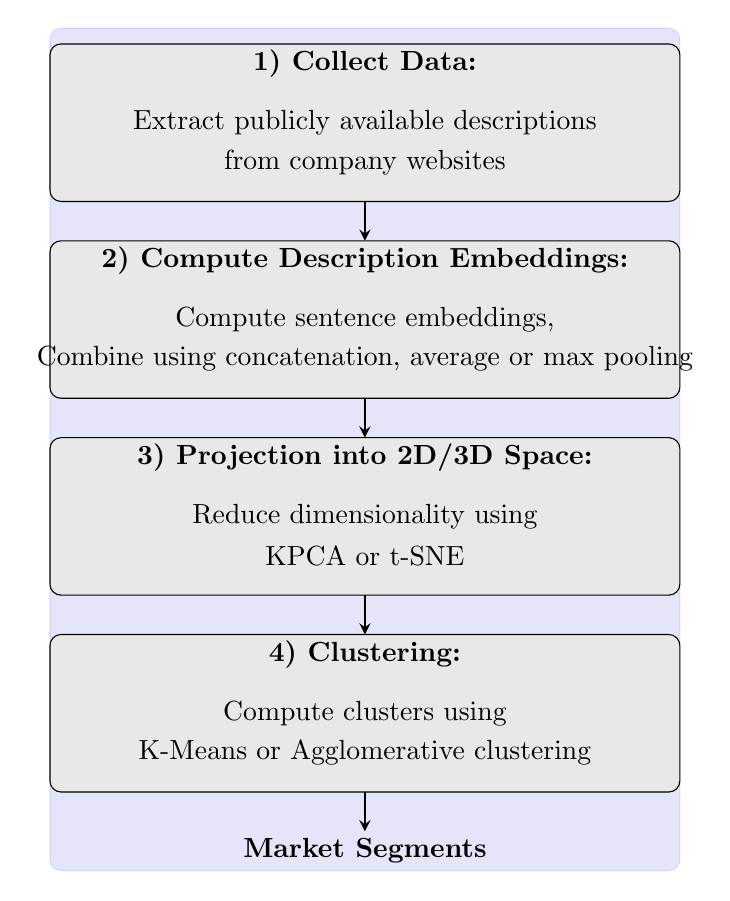
\begin{tikzpicture}
        \definecolor{lightgrey}{RGB}{232,232,232}
        \definecolor{darkblue}{RGB}{0,0,204}
        
        \draw[rounded corners, darkblue, fill=darkblue, opacity=0.1] (-4, -1) rectangle (4, 9.7);
    
        \draw[rounded corners, fill=lightgrey] (-4,7.5) rectangle (4, 9.5);
        \node[font=\bfseries] at (0, 9.25) {1) Collect Data:};
        \node at (0, 8.5) {Extract publicly available descriptions};
        \node at (0, 8.0) {from company websites};
        \draw[thick, -stealth] (0, 7.5) -- (0, 7);
    
        \draw[rounded corners, fill=lightgrey] (-4,5) rectangle (4, 7);
        \node[font=\bfseries] at (0, 6.75) {2) Compute Description Embeddings:};
        \node at (0, 6) {Compute sentence embeddings,};
        \node at (0, 5.5) {Combine using concatenation, average or max pooling};
        \draw[thick, -stealth] (0, 5) -- (0, 4.5);

        \draw[rounded corners, fill=lightgrey] (-4,2.5) rectangle (4, 4.5);
        \node[font=\bfseries] at (0, 4.25) {3) Projection into 2D/3D Space:};
        \node at (0, 3.5) {Reduce dimensionality using};
        \node at (0, 3.0) {KPCA or t-SNE};
        \draw[thick, -stealth] (0, 2.5) -- (0, 2);

        
        \draw[rounded corners, fill=lightgrey] (-4,0) rectangle (4, 2);
        \node[font=\bfseries] at (0, 1.75) {4) Clustering:};
        \node at (0, 1) {Compute clusters using};
        \node at (0, 0.5) {K-Means or Agglomerative clustering};
        \draw[thick, -stealth] (0, 0) -- (0, -0.5); 

        \node[font=\bfseries] at (0, -0.75) {Market Segments};
    \end{tikzpicture}
    \caption{Overview of our clustering pipeline.}
    \label{fig:pipeline}
\end{figure}
\pe{ s/Market Segments/Local Clusters; Market segment seems to be defined as segmenting your customer base \href{https://en.wikipedia.org/wiki/Market_segmentation}{wiki market segmentation}}



Our goal is to collect data points on companies in Saarland and cluster them to identify market segments and recommend locations for companies who plan to establish new sites, such that it supports the development of business clusters. We will present our clustering pipeline and then examine how we can use the results to provide location recommendations. 

\subsection{Identifying Related Companies through Clustering}
Figure \ref{fig:pipeline} shows a graphical representation of our general clustering pipeline, consisting of $4$ steps: $1)$ Collection of descriptions from company websites, $2)$ converting the descriptions to embeddings, $3)$ reducing the dimensionality of the embeddings, and $4)$ applying a clustering algorithm. In the following, we will examine each of these steps in detail.

\textit{$1)$ Collect Descriptions:} The traditional approach for building an economic dataset would be to gather several attributes, like revenue, number of employers, and products, for many companies in Saarland and then store each in a fixed-size vector. However, it is generally unclear which are the best attributes for representing companies. Further, it is not straightforward to encode non-numerical attributes, like products and customer base, so clustering algorithms can parse them without introducing an unwanted ordering of the attributes' values. 
Lastly, some attributes may be unavailable for some companies, meaning we would need to discard them because we require fixed-size vectors, or we would need to insert dummy values, which could lead to unwanted effects.
To address these challenges to dataset construction, we propose representing companies by the description on their websites instead of numerical attributes. The benefit of using this text data is that, since companies design their website to attract customers and investors, they include detailed information, such as their industry, products, market positioning, and customer base. Hence, we circumvent the problem of creating a targeted aggregator for specific information. This makes our approach simpler to implement and significantly more scalable \& automatable for larger target regions. 

\textit{$2)$ Compute Description Embeddings:} To achieve the fixed-size inputs required by clustering algorithms, we map each company description to an embedding that describes the data in a low-dimensional space. We rely on a sentence transformer neural network architecture to compute embeddings for each sentence in a company's description. We propose three approaches to attain a single embedding for each description: we repeatedly concatenate individual sentence embeddings until a fixed size is achieved, take the average over each feature dimension, or take the maximum over each feature dimension. The first approach, which we will call concatenation, preserves each sentence embedding's information but may introduce bias and high dimensionality, whereas the second and third approaches, which we will call average and max pooling, achieve a lower dimensionality but may discard relevant information by only keeping the average of the features or the largest features.

\textit{$3)$ Projection into 2D / 3D Space:} Although the embeddings are of much lower dimensionality than the original text data, the number of features might still be too large relative to the size of our dataset. This might invoke the curse of dimensionality, meaning that the few data points are so distant from each other in the high-dimensional space that it is impossible to derive meaningful clusters. Further, clustering data in high-dimensional space prevents the visualization of clustered data points. To avoid the course of dimensionality and to enable user-friendly visualization of our results, we will project the embeddings to 2D or 3D space using two dimensionality reduction techniques:

\emph{Kernel Principal Components Analysis} (KPCA) is a dimensionality reduction technique that computes a linear transformation that projects the data in the kernel space onto the dimensions with the highest variance, such that a non-linear transformation in the original feature space is attained. Hence, by projecting the data on the dimensions with the highest variance, KPCA preserves the most relevant information.
The \emph{t-distributed stochastic neighbor embedding} (t-SNE) technique computes a probability distribution representing the pairwise similarity between data points in the feature space and then projects the data points to a low-dimensional space according to a second probability distribution that minimizes the Kullback-Leibler divergence to the first distribution. This enables t-SNE to preserve local structures in the data accurately.
The crucial difference between KPCA and t-SNE is that KPCA computes a deterministic projection that can be applied to novel data points, whereas t-SNE does not. However, the preservation of local structures by t-SNE might be more suitable for identifying clusters.

\textit{$4)$ Clustering:} We will now present two clustering approaches that depend on the choice of dimensionality reduction technique.
If KPCA is used, we cluster the data using the $K$-Means algorithm, which, starting from $K$ randomly initialized cluster centers, assigns each data point to the nearest cluster, updates the values of the cluster centers as the mean of each data point in the cluster, and then repeats until the cluster assignments do not change anymore. We combine $K$-Means with KPCA since it returns a set of cluster centers that can be used to classify novel data points. 
If t-SNE is used, we cluster the data using agglomerative clustering, which initially assigns each data point to a separate cluster and then iteratively merges close clusters until all data points are in the same cluster. The intermediate clustering that achieves the largest overall separation between data points can then be chosen as the final clustering. The advantage of agglomerative clustering over $K$-Means is that it does not require a pre-specified number of clusters and can compute hierarchically structured clusters.
Once the clustering algorithm converges, we receive cluster labels for each company in our dataset, allowing us to predict market segments.

Although our general pipeline represents companies using their descriptions, we emphasize that our approach can also handle utilizing other features. For instance, we can include the companies' products in the encoding by computing the corresponding sentence embeddings and merging them with the description embedding using concatenation, average or max pooling. In section \MakeUppercase{\romannumeral 5}, we will investigate the results of combining company descriptions with other features.

Figure \ref{fig:clustering-analysis} depicts the clustering analysis tab of our user-interface. On the left side, users can define how the description embeddings are computed, the technique and target dimensionality of the dimensionality reduction, and the number of clusters. Additionally, users can specify a subset of additional features, including industry, products, customer base, market positioning, and revenue, which will be combined with the descriptions. After clicking "Compute clustering", the clustered data points are shown on the right side as a 2D or 3D scatter plot. Further, users can see the location and clustering assignment of all companies in our dataset on a map. When hovering the mouse over a company's data point, additional information about the company is shown, and when double-clicking the labels on the legend, only the companies of the corresponding cluster are shown.

\begin{figure}[H]
	\centering
	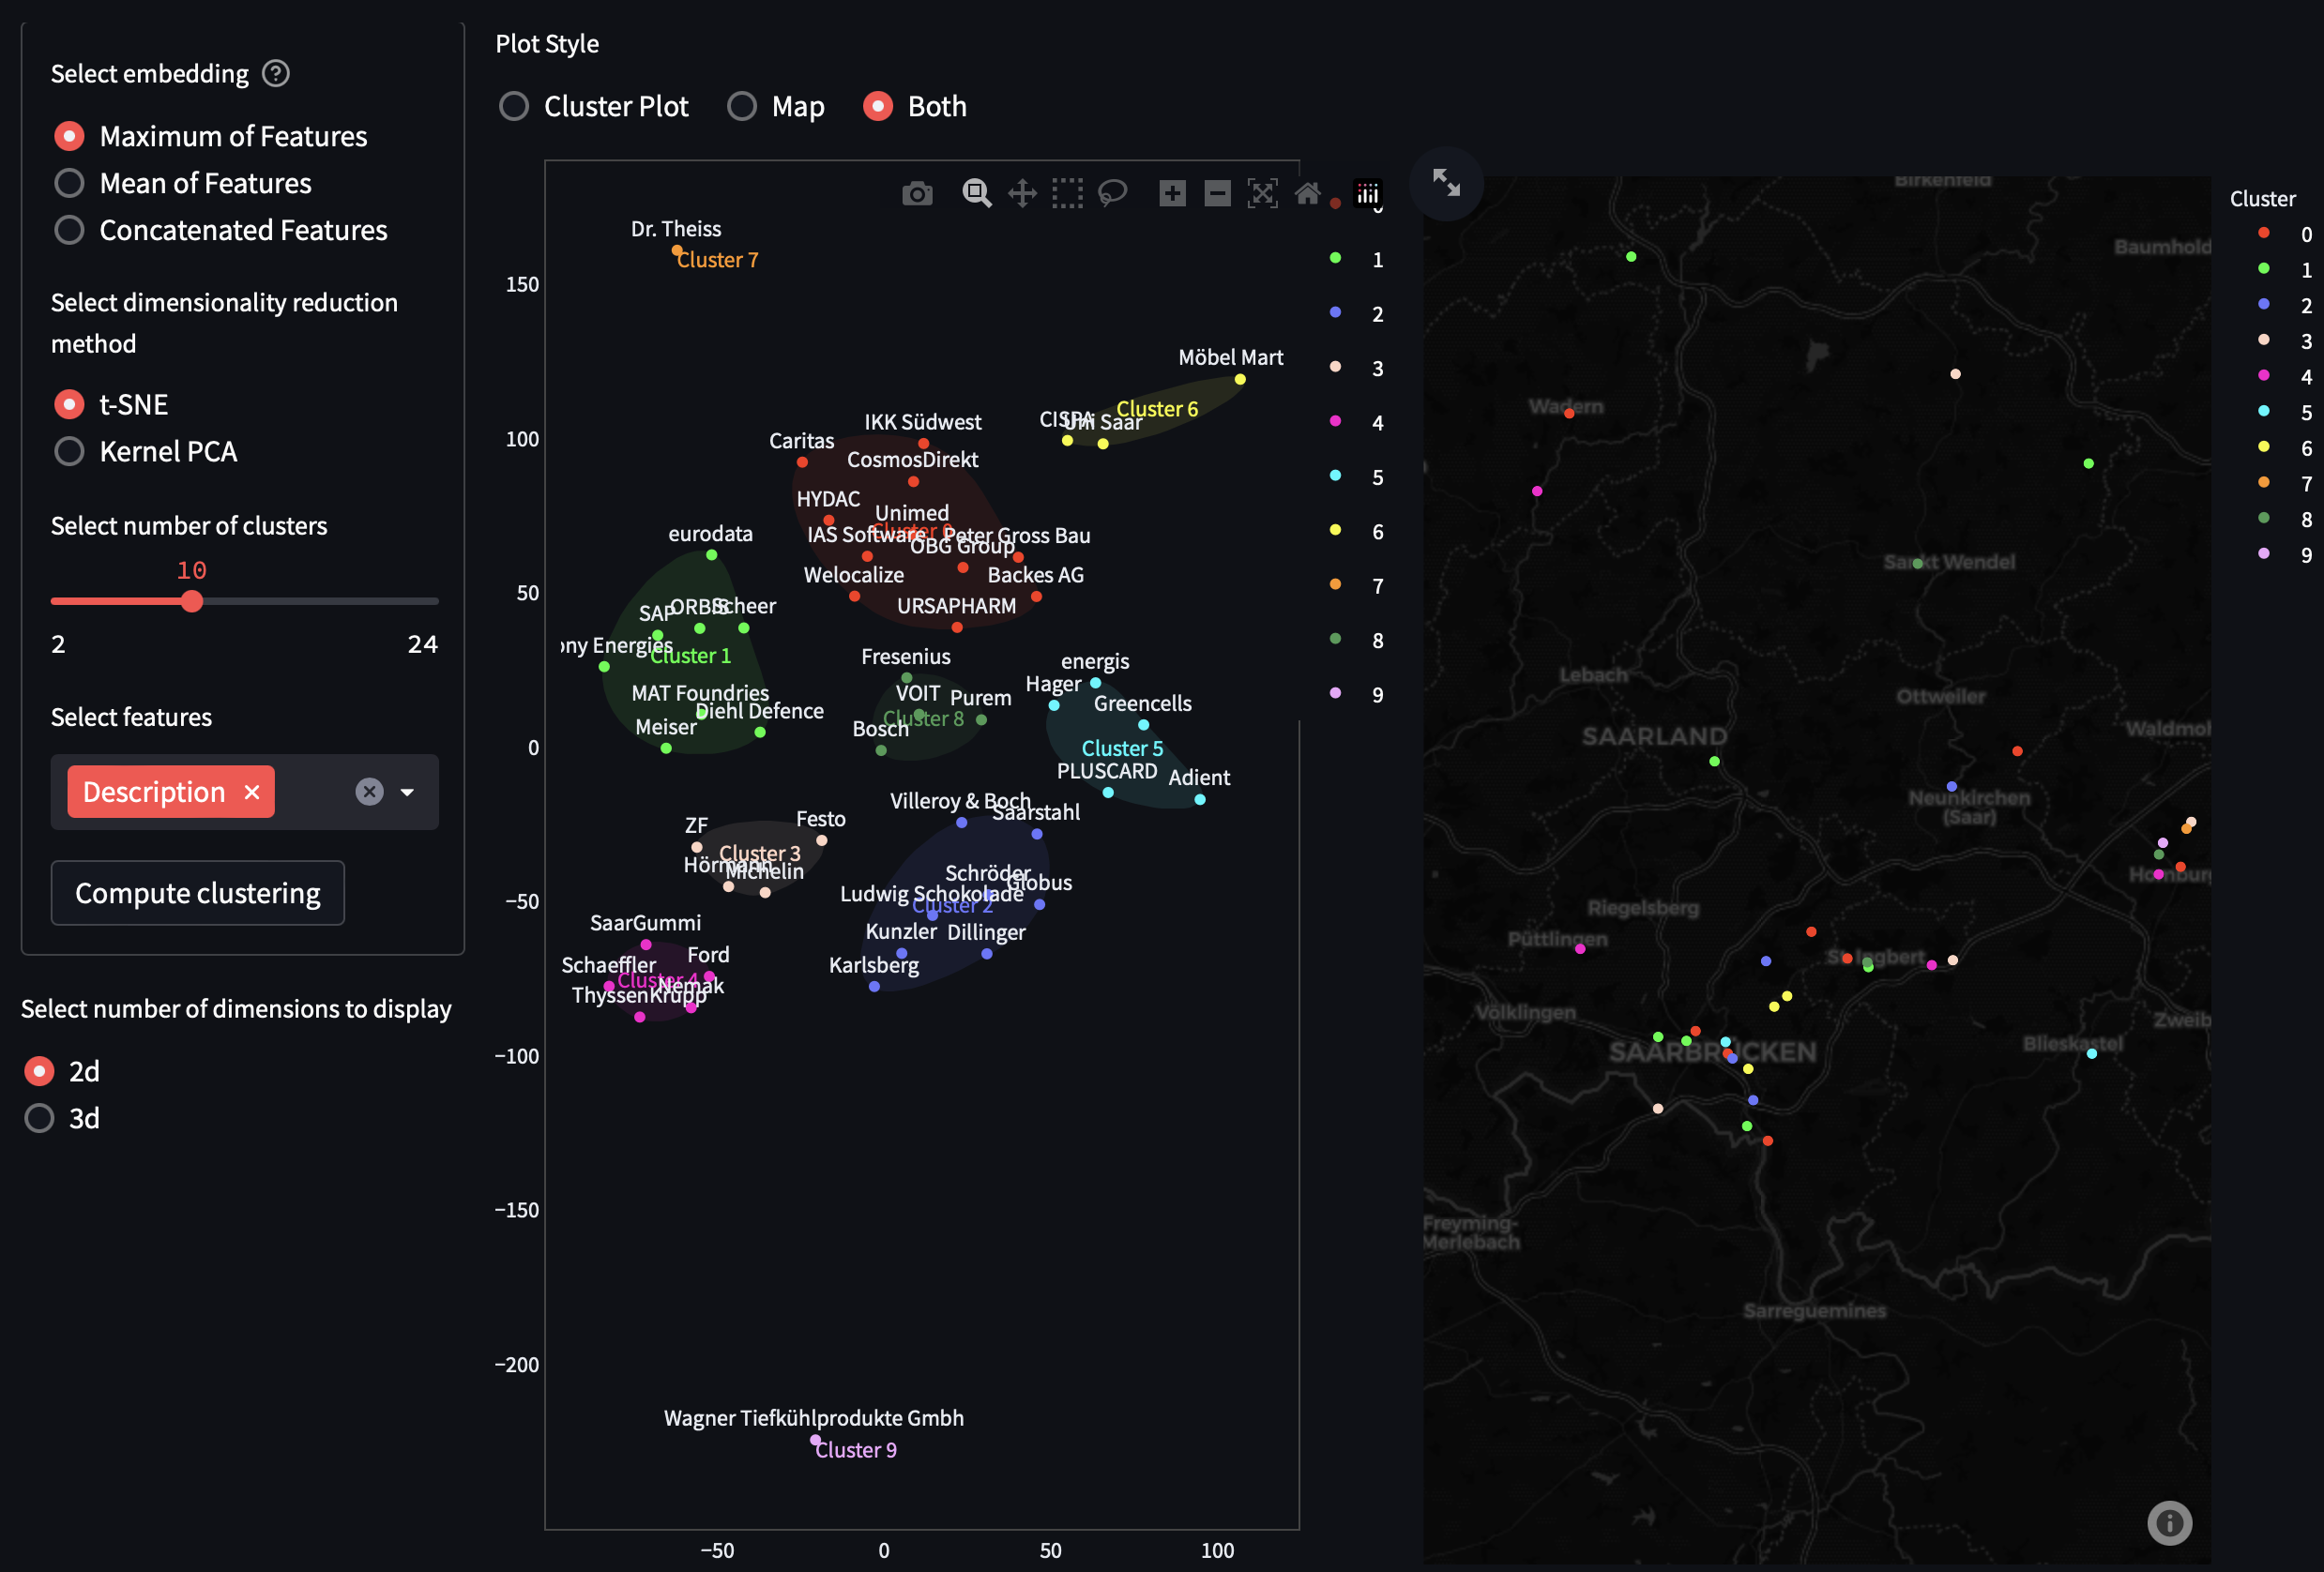
\includegraphics[width=0.5\textwidth]{figures/clustering_analysis.png}
	\caption{Clustering analysis page of our user-interface.}
	\label{fig:clustering-analysis}
\end{figure}

\subsection{Fostering Business Clusters through Location Recommendations}
We utilize parts of our clustering pipeline for recommending locations for companies seeking to establish new sites in Saarland. Given the description of the novel company, we compute an embedding using a sentence transformer and apply KPCA or t-SNE to get a low-dimensional feature vector. We then assign the feature vector to a cluster according to the $K$-Means or agglomerative clustering algorithm and then compute which company within the cluster is most similar to the novel company. Note that when using KPCA and $K$-Means, we can assign the novel data points to a pre-computed clustering, and when using t-SNE and agglomerative clustering, we compute a new clustering.
Thus, the second approach accounts for the possibility that introducing a novel company might change existing market segments, whereas the first approach does not.
Given the cluster label of the novel company, the location recommendation is to establish the new company site nearby the most similar company within the cluster, meaning we recommend placing the novel site near the most similar company acting in the same market segment, which helps to foster business clusters in Saarland.

Our user-interface offers a dedicated tab for location recommendations. In figure \ref{fig:location-recommendation-input}, we see the text boxes where users can provide their company's name and description. Additionally, users can specify their company's industry, products, customer base, market position, and revenue, which can be used in the location recommendations. After clicking "Submit", users are shown the output depicted in figure \ref{fig:location-recommendation-output}. The table at the top shows the names and features of the companies in the cluster to which the user's company was assigned. The scatter plot at the bottom left shows the clustered data points, where the point of the user's company is highlighted. Lastly, the map at the bottom right displays the location of the novel company's cluster members and the distances between them. The user can also overlay a heatmap that shows the similarity between his company and all other companies in our dataset.

\begin{figure}[H]
	\centering
	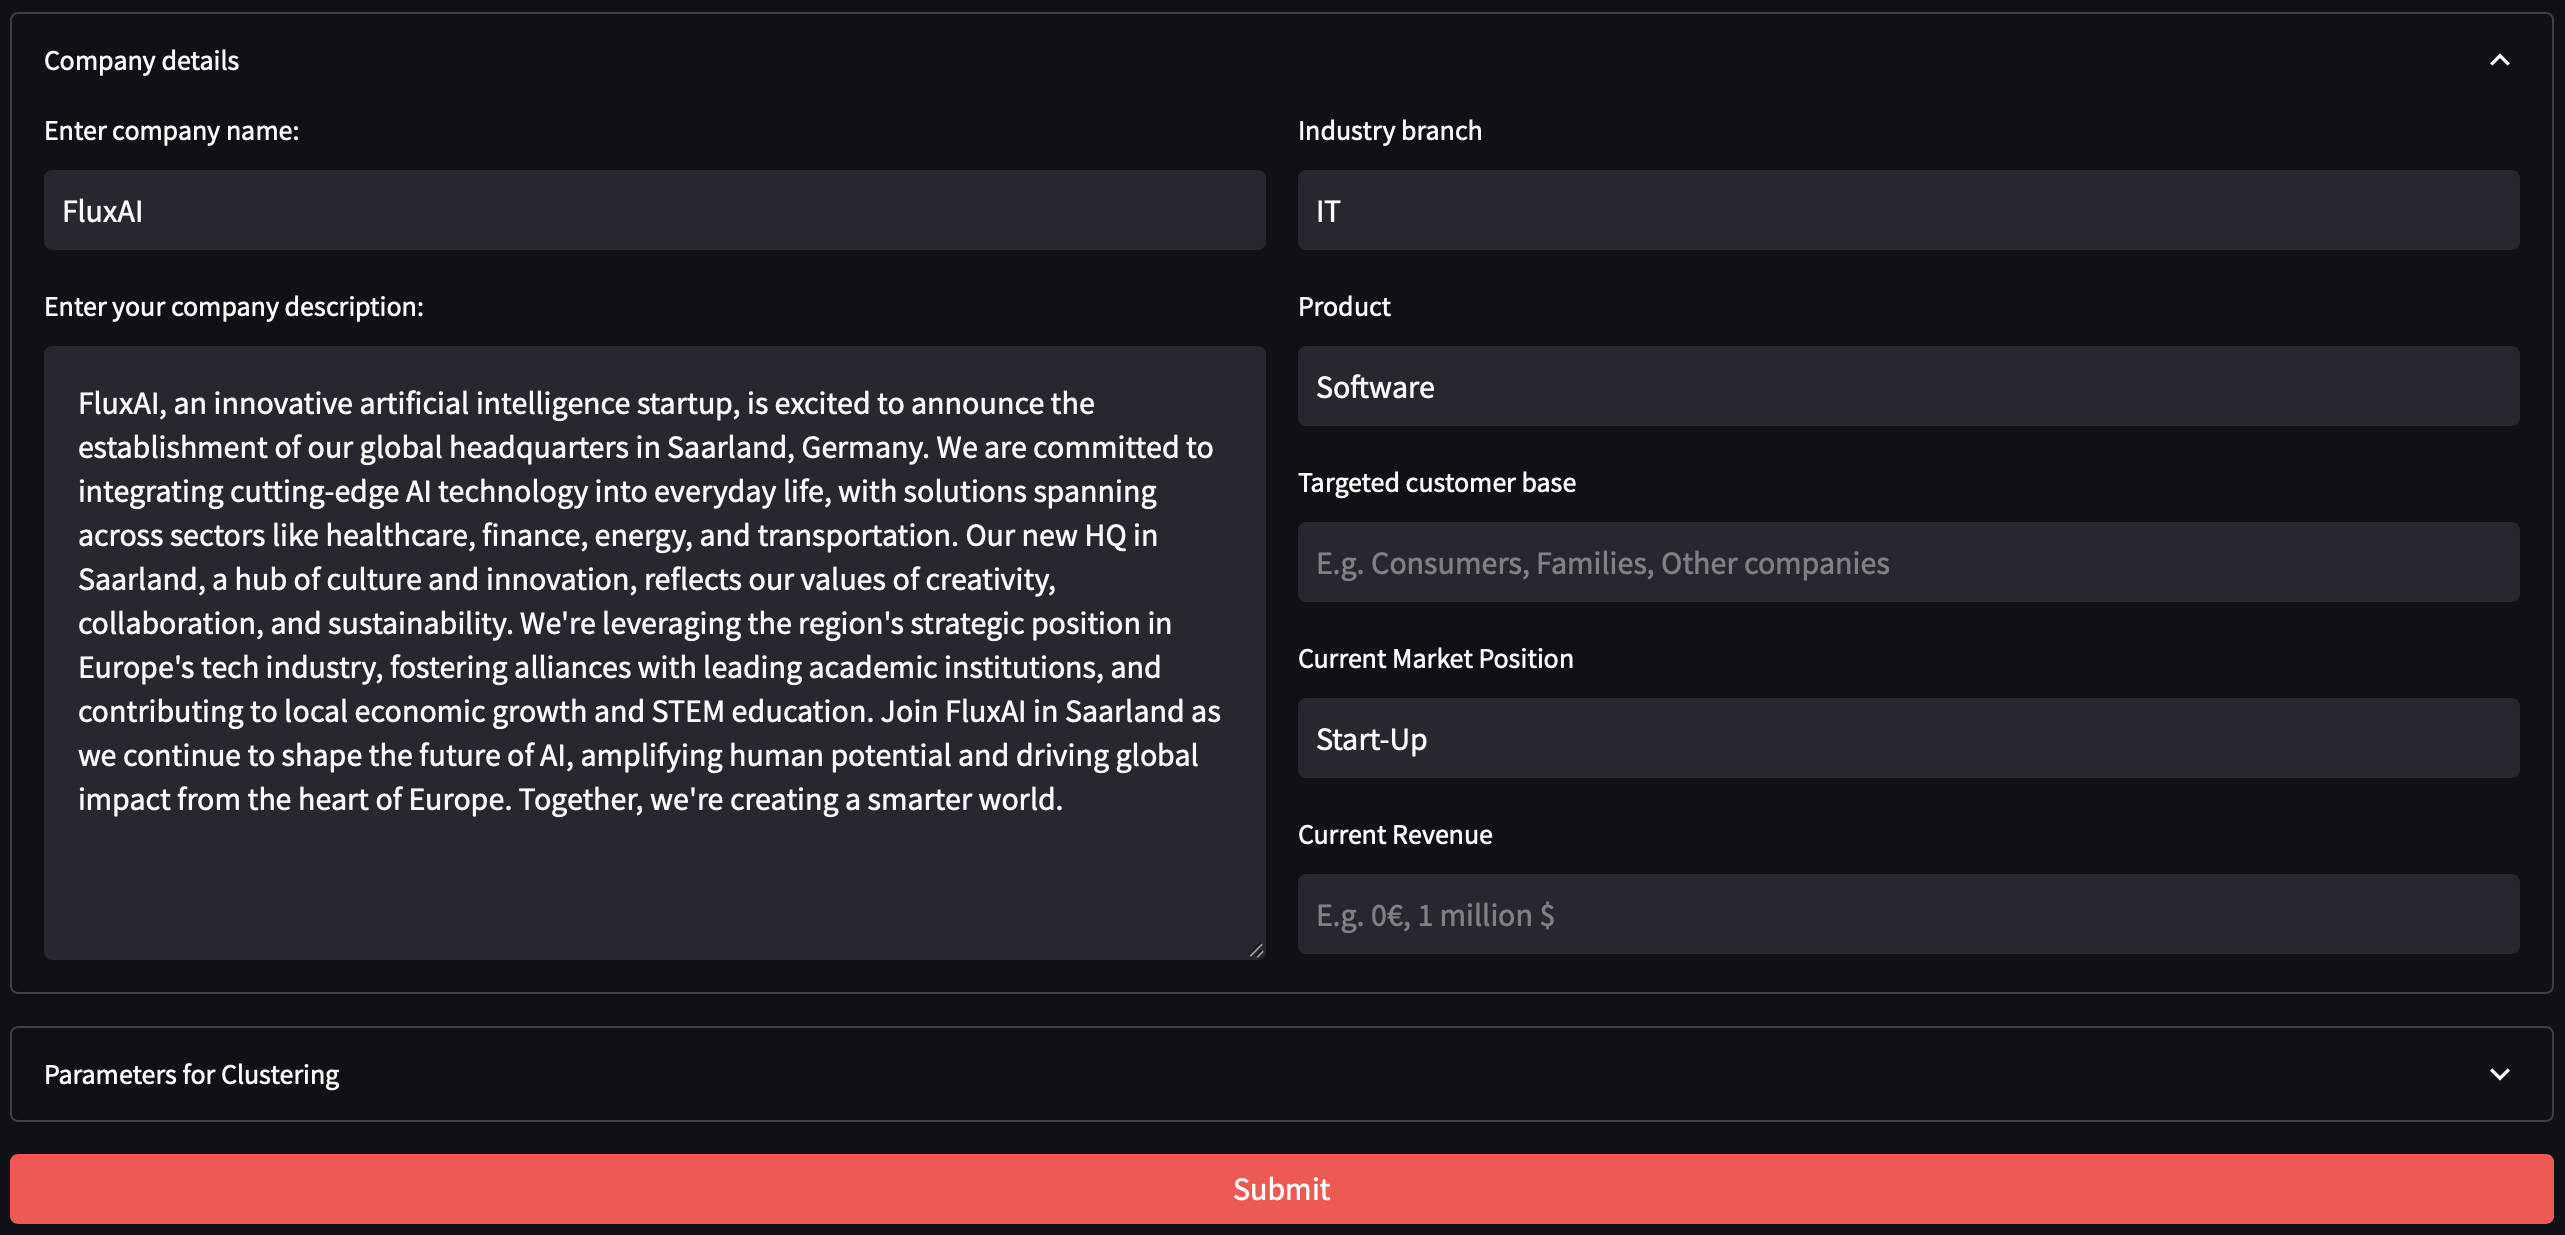
\includegraphics[width=0.5\textwidth]{figures/location_recommendation_input.png}
	\caption{Input to the location recommendation feature of our user-interface.}
	\label{fig:location-recommendation-input}
\end{figure}
\begin{figure}[H]
	\centering
	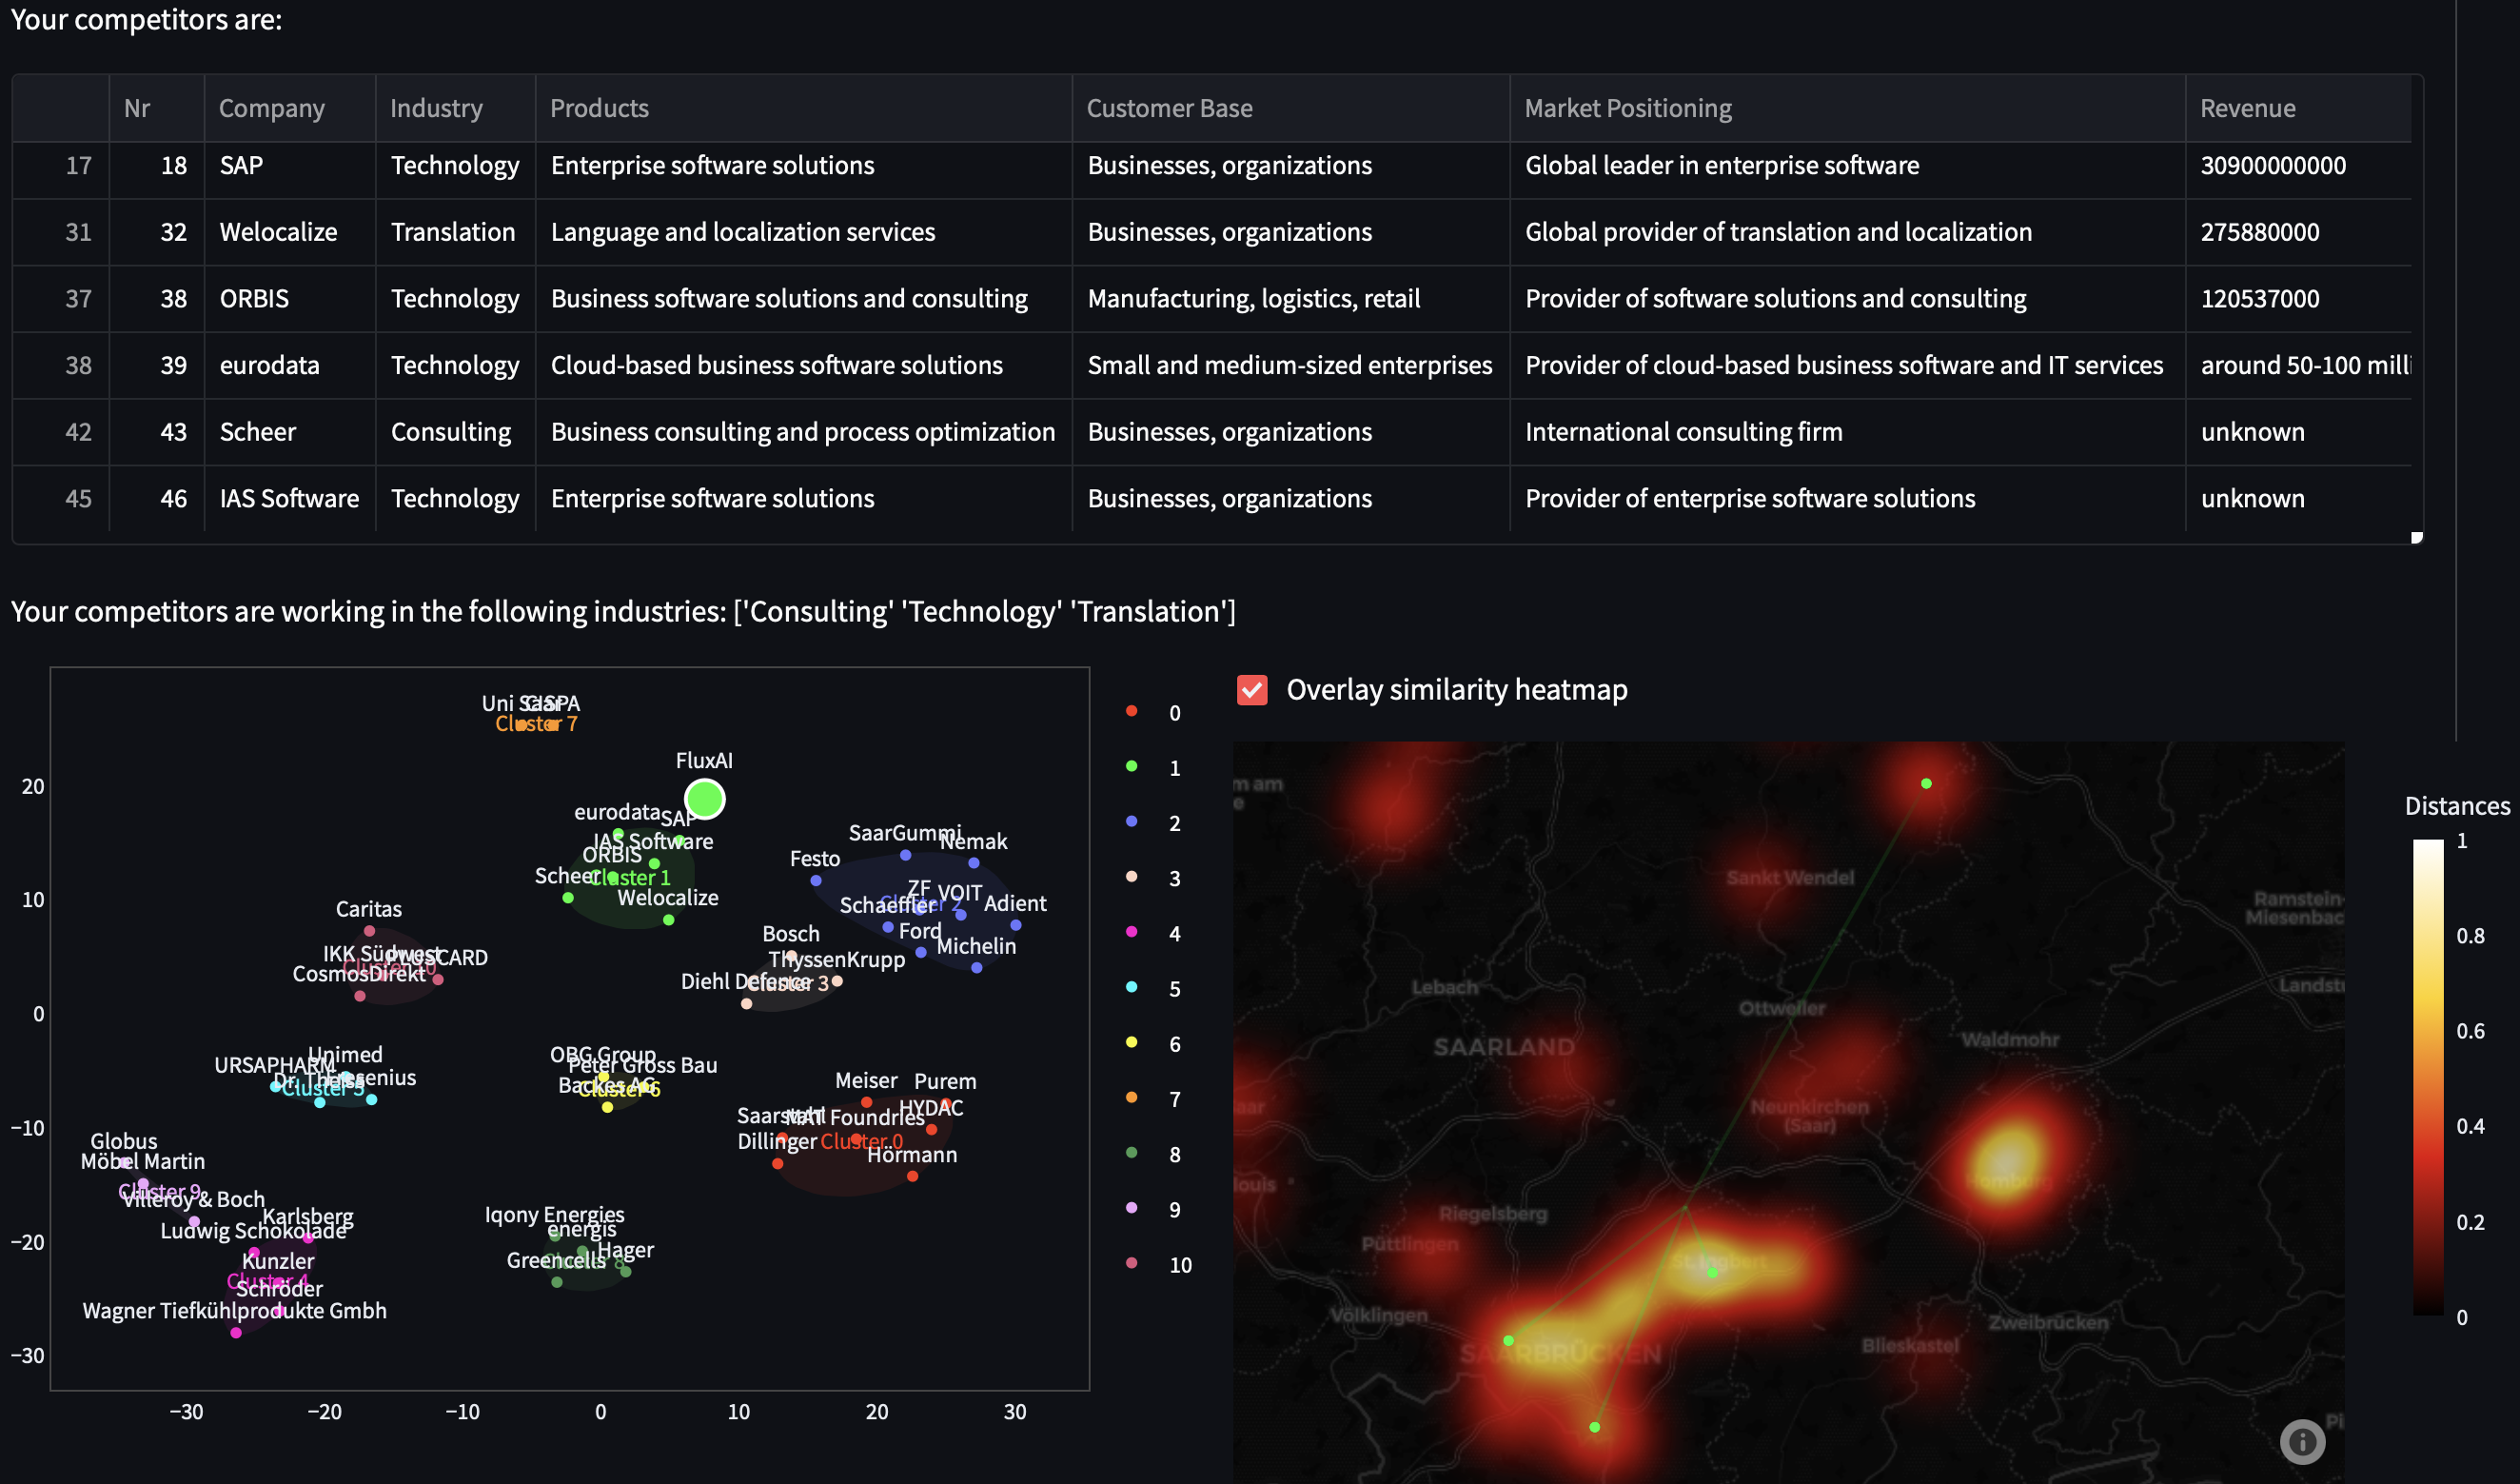
\includegraphics[width=0.5\textwidth]{figures/location_recommendation_output.png}
	\caption{Output of the location recommendation feature of our user-interface.}
	\label{fig:location-recommendation-output}
\end{figure}

\section{Experiments}
To build our dataset of company descriptions, we manually extracted the descriptions of $50$ of the largest companies in Saarland. When a description was only available in German, we translated it to English using the online translator DeepL~\cite{deepl}. A list of all companies in our dataset can be found in the appendix \ref{sec:appendix-companies}.

For the purpose of the experimental evaluation, we conducted the data collection manually. As our target region was very narrow, this was easily feasible. However, in the future, we might create a simple HTML scraper to scale our approach to larger regions. To test our location recommendation feature, we created company descriptions using GPT-4 \cite{chatgpt}.

Additionally, we evaluate the impact of providing additional features to the clustering pipeline, for which we also gathered the features industry, products, customer base, market positioning, and revenue of each company.

We utilize the popular pre-trained sentence transformer model "all-MiniLM-L6-v2" from the HuggingFace hub~\cite{sentence-transformer-model} to compute sentence embeddings for each description. An embedding for the full description is then attained using our concatenation, average, or max pooling approach. When using additional features, we compute embeddings for each feature and combine them with the description embedding in the same way the individual sentence embeddings were combined.
Afterward, the embeddings are projected into 2D or 3D space using KPCA or t-SNE. We chose suitable hyperparameters for KPCA by conducting a grid search over the values $\textit{kernel} = \{\textit{radial basis function}, \textit{sigmoid}, \textit{linear}, \textit{polynomial} \}$ and $\textit{gamma} = \{0.03, 0.032, 0.034, \dots, 0.05\}$, where we found the best values to be $\textit{kernel} = \textit{polynomial}$ and $\textit{gamma} = 0.05$. For t-SNE, we manually fine-tuned the perplexity hyperparameter until we achieved a suitable separation of data points.

To choose the number of clusters for $K$-Means, we started with $K = \sqrt{N}$, where $N$ is the size of the dataset, and then increased $K$ until the clustering aligned with our expectations. For agglomerative clustering, we chose the final number of clusters through visual inspection of the dendrogram returned by the algorithm.

\section{Results}
\begin{figure}[H]
	\centering
	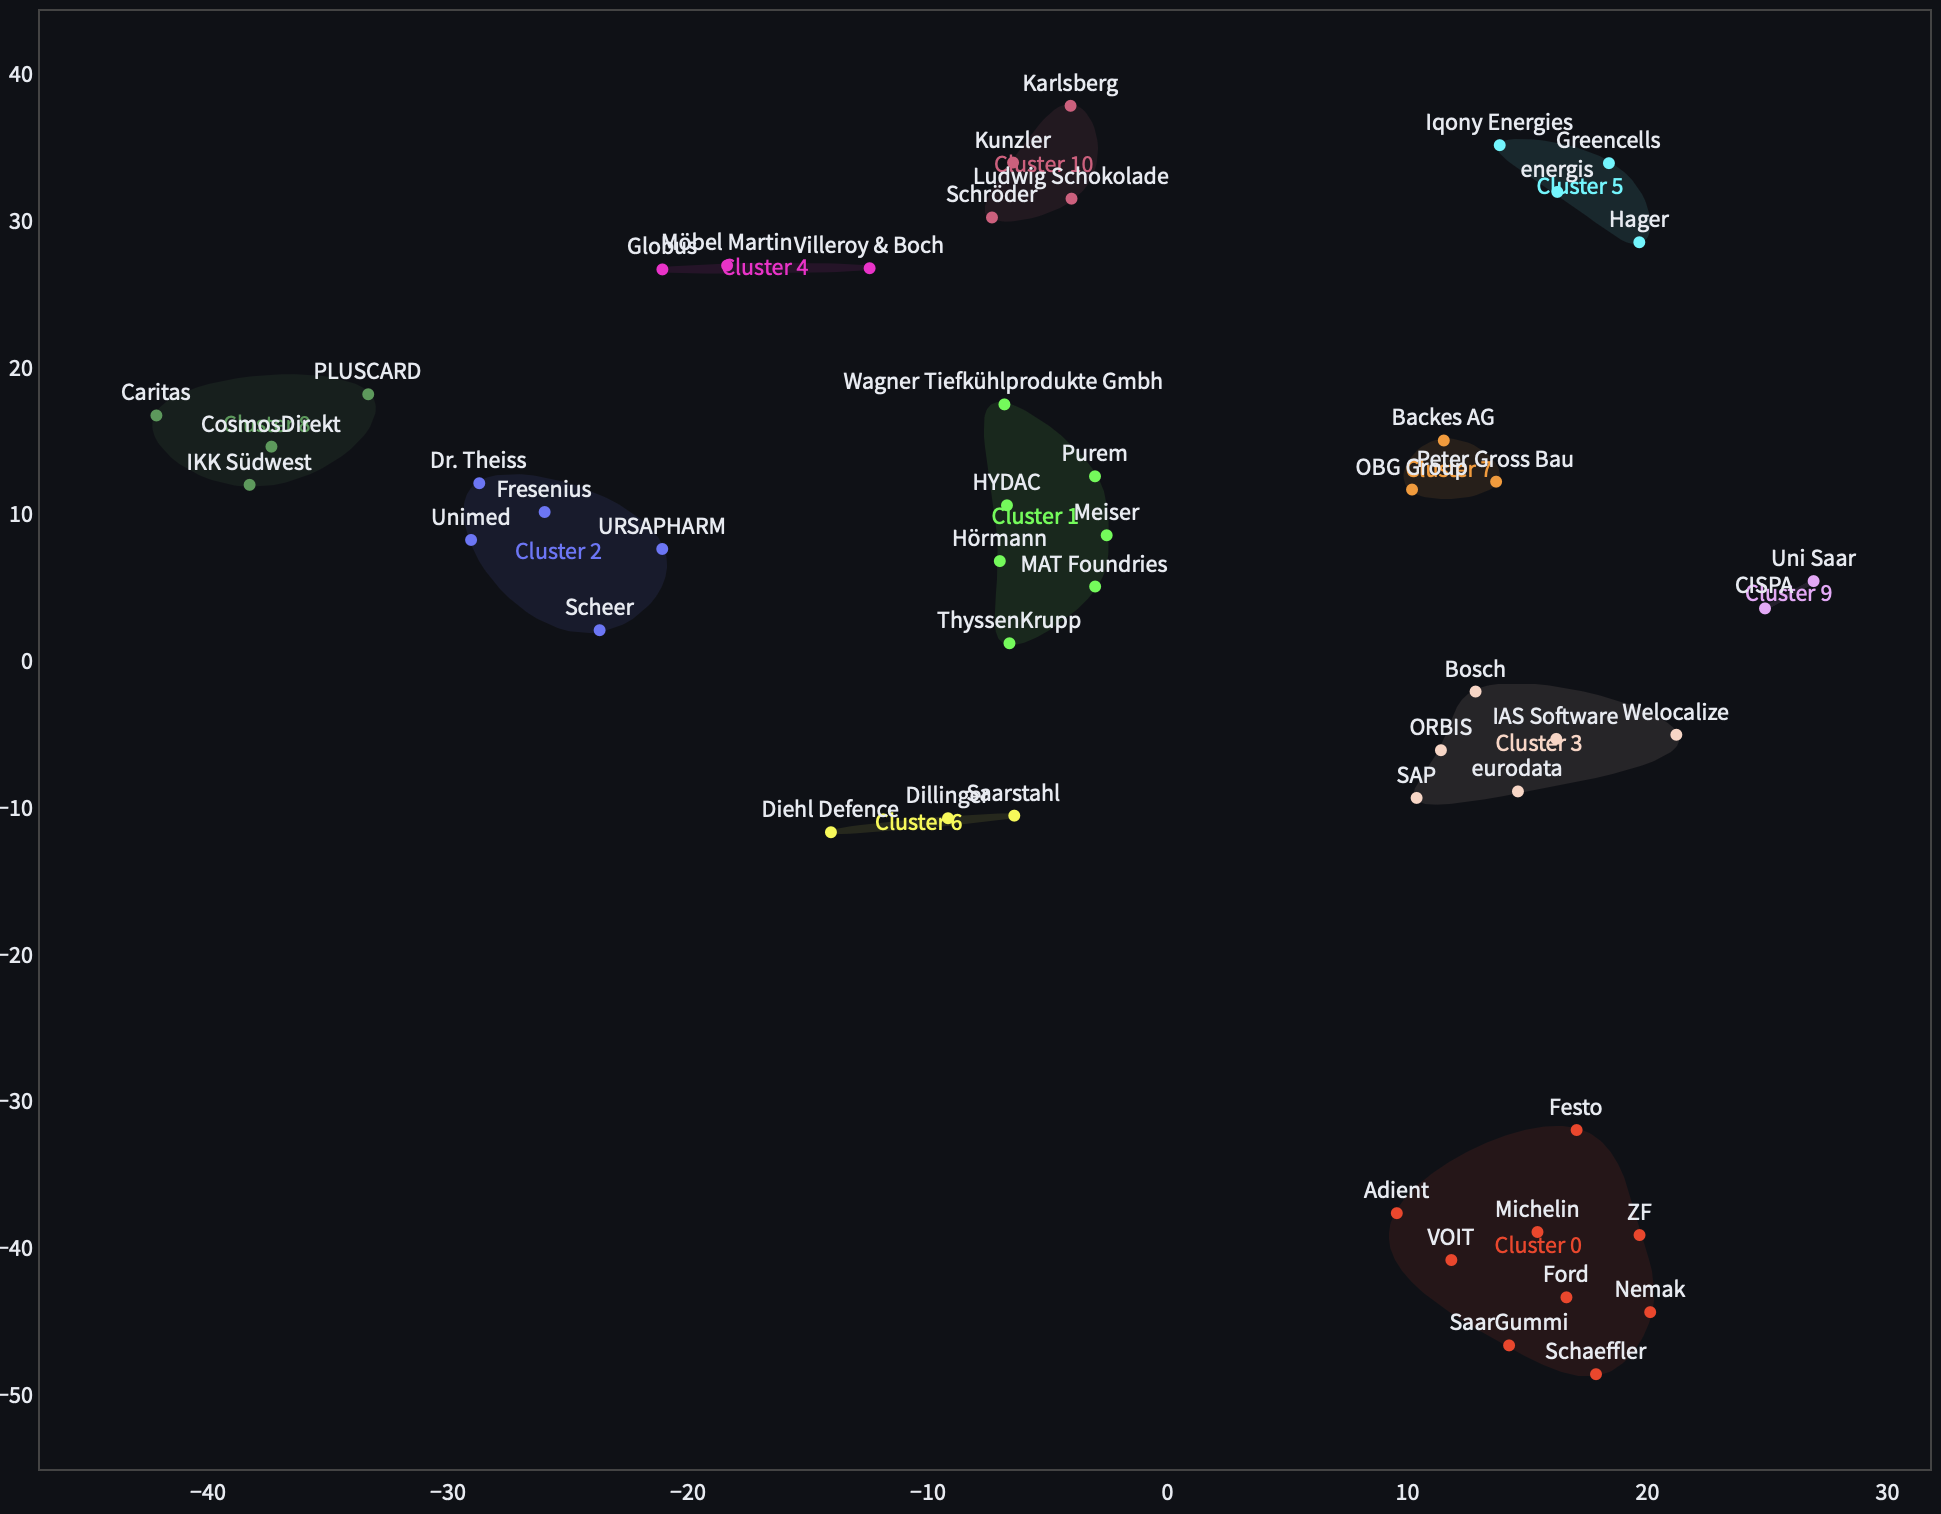
\includegraphics[width=0.5\textwidth]{figures/clustering_results.png}
	\caption{Clustering of company descriptions using t-SNE and Agglomerative clustering. The company descriptions and industries were used as features.}
	\label{fig:t-sne-agglomerative}
\end{figure}

In the following, we will investigate the results of the best-performing configuration of our clustering and location recommendation system. These results were obtained using the following configuration: the description embeddings were computed using max pooling, the embeddings were projected into 2D space using t-SNE, and the clustering was achieved using agglomerative clustering. We also used the companies' industry as an additional feature.
We found that this configuration yields the most sensible clusters and location recommendations. Figure \ref{fig:t-sne-agglomerative} displays the resulting clustered data points.

\subsection{Clustering}
\label{sec:clustering-results}
In the following, we analyze each of the found clusters and interpret them with respect to potential market segments:
\begin{itemize}
	\item \textit{Cluster 0 (red)}: This cluster consists of automotive manufacturers and suppliers, such as Ford and Michelin. Hence, we follow that this cluster represents the automotive industry market segment.
	
	\item \textit{Cluster 1 (light green)}: The steel industry companies MAT Foundries, ThyssenKrupp, and Meiser are part of this cluster. Further, cluster members are companies like Hörmann and HYDAC, which also offer products manufactured from steel. Accordingly, we assign this cluster to the steel products market segment. The food manufacturer Wagner can be considered misclassified, as it should be contained in Cluster 10.
	
	\item \textit{Cluster 2 (dark blue)}: We attribute this cluster to the healthcare market segment since it contains the medicine manufacturers Dr. Theiss and URSAPARM, Fresenius, which produces dialysis machines, and Unimed, which provides accounting services for hospitals. Note that the IT consulting firm Scheer can be considered misclassified and should be added to Cluster 3.
	
	\item \textit{Cluster 3 (beige)}: This cluster contains the IT companies SAP, ORBIS, eurodata, IAS Software, and Welcoalize, representing the IT products and IT consulting market segment. Although the cluster member Bosch is not an IT company, it also offers software products, so we do not consider it misclassified.
	
	\item \textit{Cluster 4 (purple)}: This cluster consists of the companies Globus, Möbel Martin, and Villeroy\&Boch, which offer very different products but are all large retailers. Hence, we assign this cluster to the retail market segment. 
	
	\item \textit{Cluster 5 (light blue)}: The energy provider energis and the energy service providers Iqony Energies and Greencells are contained in this cluster. Hager is also a cluster member specializing in electrical installation and energy distribution. Accordingly, we infer that this cluster represents the energy market segment.
	
	\item \textit{Cluster 6 (yellow)}: We assign this cluster to the steel production market segment since it contains the steel manufacturers Dillinger and Saarstahl. The defense company Diehl Defence can be considered misclassified, as it should be in a single cluster because it is the only defense company in our dataset.
	
	\item \textit{Cluster 7 (orange)}: This cluster consists of the construction companies Backes AG, Peter Gross Bau, and OBG Group, so it represents the construction work market segment.
	
	\item \textit{Cluster 8 (dark green)}: Because the insurance companies CosmosDirekt and IKK Südwest are part of this cluster, it could indicate the insurance market segment. However, this cluster also contains the healthcare service provider Caritas, which should be in Cluster 2, and the credit card provider PLUSCARD.
	
	\item \textit{Cluster 9 (lavender)}: The only two members of this cluster are Uni Saar and CISPA, making it representative of the academia market segment.
	
	\item \textit{Cluster $10$ (pink)}: This cluster consists of food producers such as Kunzler and Ludwig Schokolade, and thus it represents the food market segment.
\end{itemize}
We conclude that our clustering methods are effective since we saw that each of the 11 clusters mostly contained similar companies, allowing us to infer various market segments.

\subsection{Comparison to Clusters Identified by Other Work}

As mentioned \cite{saarlandeco2} also identified clusters for the region of Saarland. We compare their results (\cite{saarlandeco2}, Table 4, p. 1226) with the output of our pipeline:


\begin{itemize}
	\item \textit{Coal and mining industries}: With the decline of coal mining in recent years, there are no more coal mines in Saarland. As the last one closed in 2012, this cluster does not exist anymore. 
	\item \textit{Metal industry}: Covered by cluster 1 (light green) and cluster 6 (yellow).
	\item \textit{Automobile industry}: Covered by cluster 0 (red).
	\item \textit{Energy sector}: Covered by cluster 5 (light blue).
	\item \textit{Information and communication technology}: Covered by cluster 3 (beige).
	\item \textit{Biotechnology and nanotechnology}: Covered by cluster 2 (dark blue).
\end{itemize}

One can see that the results of our pipeline do agree with the general sectors identified by \cite{saarlandeco2}. However, our approach did lead to more fine-grained separation. Additionally, we identified sectors not covered in their work, such as cluster 7, which represents the construction work market segment. However, these sectors usually do not contribute significantly to the region's economy, which is probably why they are not mentioned in \cite{saarlandeco2}. In summary, the output of our pipeline matches very well with traditionally identified clusters.

\subsection{Location Recommendation}
To test our location recommendation system, we generated descriptions for four fictional German companies with vastly different characteristics:
\begin{itemize}
	\item \textit{FluxAI}: A young artificial intelligence start-up with ambitious goals of revolutionizing healthcare, finance, energy, and transportation.
	\item \textit{ABC Auto}: A well-established automotive manufacturer offering a wide range of cars focusing on sustainability.
	\item \textit{Bratwurst Bliss}: A hot dog manufacturer that values traditional sausage making and locally sourced ingredients.
	\item \textit{PanzerTech}: A weapons manufacturer with a wide spectrum of products, from armored vehicles to cybersecurity solutions.
\end{itemize}

For FluxAI, our system recommends placing the new site close to CISPA, which is sensible since CISPA is a world leader in information security research, which also includes artificial intelligence, and thus knowledge transfer between both companies could be highly beneficial. It also makes sense that our system did not recommend locating FluxAI near IT companies with a more commercial focus, like SAP, since they primarily work on existing technology instead of revolutionary innovations.
For ABC Auto, the location recommendation is to establish a new site close to VOIT, which specializes in manufacturing car components with a focus on hybrid and electric cars. Thus, placing ABC Auto near VOIT would allow ABC Auto to source parts for its hybrid and electric cars from a company nearby, leading to a more robust supply chain.
For Bratwurst Bliss, the system recommends settling near the meat producer Kunzler, which could lead to knowledge transfer regarding sausage-making.
Lastly, our system recommends placing PanzerTech's new site close to Diehl Defence, corresponding to the only weapons manufacturer in our dataset. Hence, this shows that our system does not need a large number of samples from each market segment to give reasonable location recommendations.

We conclude that our location recommendation system can reliably identify companies in our dataset with similar characteristics to companies seeking to establish sites in Saarland and thus can be used to foster the development of business clusters.

\subsection{Limitations}
We observed in subsection \ref{sec:clustering-results} that a small number of companies were assigned to the wrong clusters. These companies mostly belonged to sectors that are underrepresented in our dataset, such as defense and financial services, so we would likely achieve more concise cluster assignments if we added more companies from these sectors to our dataset.

Another reason for invalid cluster assignments could be that our utilized sentence transformer was not fine-tuned for company descriptions, so that it could have produced inaccurate embeddings for some descriptions. Further, projecting the embeddings into 2D or 3D space could also cause inaccurate cluster assignments due to a large loss of information. Projecting the embeddings into higher dimensions might avoid this information loss, yet it would complicate or prevent a user-friendly visualization of the clustering results.

\section{Conclusion}
The goal of this project was to collect data on companies in Saarland and apply clustering algorithms such that the results can be used to identify market segments and give location recommendations for novel companies such that business clusters are fostered.

To circumvent the challenges of feature selection and encoding non-numerical features, we represented companies by their publicly available descriptions. We leveraged state-of-the-art language models to transform this highly informative text data into machine-readable embeddings. Lastly, we utilized two approaches to project the embeddings into low-dimensional space where clustering can be applied.
Our methods allowed straightforwardly including other standard company attributes, such as industry, customer base, market positioning, and revenue. 
To make location recommendations, we passed the descriptions and features of novel companies to our clustering pipeline and then recommended establishing new sites next to the most similar companies in our dataset.

A qualitative evaluation of our methods has shown that they can reliably cluster similar companies, which allowed us to infer market segments in Saarland. Further, our location recommendation system demonstrated its capability of identifying similar companies, given the description of a new company, independently of the total number of similar companies in the dataset.

To allow end-users to leverage our methods, we implemented a user-friendly interface with many functionalities, such as visualizing the clustered data points, modifying the clustering parameters, showing the location of companies, and giving detailed and interpretable location recommendations.

We see many opportunities for future work. Collecting data from more companies in Saarland could improve the clustering results, although the number of (large) companies in Saarland is limited. Thus, applying our methods to larger economies would be of great interest. This would also allow more comparisons to traditionally identified clusters. Further, fine-tuning our language models using text data from the business sector might lead to more expressive embeddings. To achieve this efficiently, an automated aggregation system could be developed. As we rely on publicly available websites, this would be easily possible without relying on 3rd party services.
To this end, we have demonstrated the feasibility and potential of applying language models to economic analysis.


\bibliographystyle{IEEEtran}
\bibliography{bibliography}

\newpage
\appendix
\nm{Upload all \LaTeX{} files to overleaf when its done since they want a link!}
\subsection{Link to Code}
\url{https://github.com/nicola-mueller/LM-based_Company_Clustering}

\subsection{Link to Overleaf}


\subsection{Companies in our Dataset}
\label{sec:appendix-companies}

We list the $50$ Saarland companies in our dataset:
\begin{multicols}{2} \begin{itemize}
	\item ZF
	\item Saarstahl
	\item Dillinger
	\item Bosch
	\item Festo
	\item Ford
	\item Schaeffler
	\item Fresenius
	\item Wagner
	\item Villery\&Boch
	\item Michelin
	\item ThyssenKrupp
	\item Hager
	\item Purem
	\item SaarGummi
	\item VOIT
	\item Meiser
	\item SAP
	\item Nemak
	\item Peter Gross Bau
	\item OBG Group
	\item URSAPHARM
	\item Hörmann
	\item Kunzler
	\item Diehl Defence
	\item HYDAC
	\item Backes AG
	\item Karlsberg
	\item Globus
	\item Caritas
	\item Uni Saar
	\item Welocalize
	\item Möbel Martin
	\item IKK Südwest
	\item Dr. Theiss
	\item Unimed
	\item CosmosDirekt
	\item ORBIS
	\item eurodata
	\item energis
	\item CISPA
	\item Greencells
	\item Scheer
	\item Iqony Energies
	\item PLUSCARD
	\item IAS Software
	\item Ludwig Schokolade
	\item MAT Foundries
	\item Adient
	\item Schröder
\end{itemize}\end{multicols}


\end{document}
